\chapter{Projektmanagement}
\section{Allgemeines}
Um ein Projekt ordentlich zu planen und durchzuführen, um häufige Fehler zu vermeiden und maximale Produktivität zu gewährleisten ist ein Projektmanagement unumgänglich. Aus diesem Grund haben wir uns für die Agile Softwareentwicklungsmethode Kanban entschieden. Die Umsetzung erfolgt mit täglichen, morgendlichen Meetings wo wir Absprachen zum Geschafften am Vortag und Ziele des Tages halten um uns so am Laufenden zu halten. Auch wurde als Kanban-Board das in GitLab integrierte Issue-Board verwendet, um den Arbeitsfortschritt laufend zu dokumentieren und um Probleme klar aufzuzeigen.\\

\begin{figure}[h]
	\centerline{
		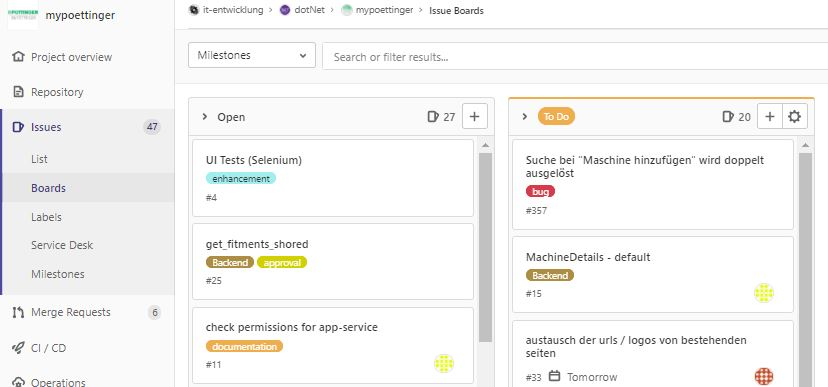
\includegraphics[width=1\textwidth, frame]{./grafiken/GitLab_issue_Board.JPG}
	}
	\vskip0pt
	\caption{Das Issue-Board in GitLab}
\end{figure}


Im November 2019 haben wir begonnen uns mit der Firma Pöttinger Landtechnik GmbH und unserem Betreuer Herrn Rainer Sickinger abzusprechen.\\
Anschließend erfolgte die Erstellung des Pflichtenheftes, welches den Start der Projektarbeit darstellte. Finalisiert wurde das Pflichtenheft in Zusammenarbeit mit \ThPartnerPersonName \ in einem Meeting.\\
Im Juli 2020 begannen wir bei der Firma Pöttinger mit der Arbeit. Projektabschluss war im Februar 2021, wo der letzte Teil implementiert wurde.

\section{Meilensteine}
\renewcommand\tabularxcolumn[1]{>{\centering\arraybackslash}m{#1}}
\begin{table}[H]
	\centering
{\rowcolors{2}{gray!20}{gray!10}
	\setlength{\arrayrulewidth}{1pt}
\begin{tabular}[h]{|l|m{8cm}|p{2.5cm}|p{2.5cm}|}
	\hline
	\rowcolor[gray]{.6}	\textbf{\#} & \textbf{Meilenstein} & \textbf{SOLL-Fertigstellung} & \textbf{IST-Fertigstellung} \\
	\hline
	1 & Erstellung eines statischen Registrierungsformulars & Juli 2020 & Juli 2020 \\
	\hline
	2 & Aufbau einer dynamischen Internationalisierungsmöglichkeit & Juli 2020 & Juli 2020 \\	
	\hline
	3 & Erweiterung durch Komfortfeatures zur schnelleren/benutzerfreundlicheren Registrierung & Juli 2020 & Juli 2020 \\
	\hline
	4 & Schaffen von Login/Logout-Möglichkeiten & Juli 2020 & Juli 2020 \\	
	\hline
	5 & Entwicklung einer dynamisch generierten Registrierungsformulars & Juli 2020 & Juli 2020 \\	
	\hline
	6 & Gestaltung und Implementierung einer Profilseite zur Einsicht und Bearbeitung der Daten, sowie An-/Abmeldung zum Newsletter & Juli 2020 & Juli 2020 \\	
	\hline
	7 & Entwicklung des Maschinenparks & Juli 2020 & Juli 2020 \\	
	\hline
	8 & Einbinung der Module in die Startseite (Produktpalette / Maschinensuche / Konfigurator / PÖTSEM) & August 2020 & August 2020 \\	
	\hline
	9 & Implementierung der Startseite & August 2020 & August 2020 \\	
	\hline
	10 & CI/CD Pipeline & Februar 2021 & Februar 2021 \\	
	\hline	
	11 & Diplomarbeit fertig verfasst & März 2021 & März 2021 \\
	\hline
\end{tabular}
}
\caption{Meilensteine}
\end{table}
Die definierten Meilensteine sind teils kleine Schritte, um den Grundstock für das weiterarbeiten zu ermöglichen. Da das Projektteam den gesamten Juli durcharbeitete, war es möglich, viele der Meilensteine in diesem einem Monat zu erreichen. 

%\section{Soll-Ist-Vergleich des Aufwandes}
%In der darunter stehenden Tabelle wird der geschätzte und der tatsächliche Aufwand in Stunden verglichen. 